%==============================================================================
%  Dhruv Kamdar - India CV  (Analytics | AI | Finance)
%  Single-column, ATS-parser-safe, single page A4.
%  Compile with: pdflatex Dhruv_Kamdar_CV_India.tex   (run twice)
%  Requires profile.png in the same folder.
%==============================================================================
\documentclass[a4paper,10pt]{article}

\usepackage[top=0.75cm,bottom=0.65cm,left=1.5cm,right=1.5cm]{geometry}
\usepackage[T1]{fontenc}
\usepackage[utf8]{inputenc}
\usepackage[scaled=0.92]{helvet}
\usepackage{mathptmx}
\renewcommand{\familydefault}{\sfdefault}
\usepackage{xcolor}
\usepackage{tikz}
\usepackage{graphicx}
\usepackage{enumitem}
\usepackage{array}
\usepackage{fontawesome5}
\usepackage[letterspace=150]{microtype}
\usepackage{hyperref}

\hypersetup{colorlinks=true,urlcolor=black,linkcolor=black,pdfborder={0 0 0},
            pdftitle={Dhruv Kamdar - CV},pdfauthor={Dhruv Kamdar},
            pdfsubject={Data, AI and Finance Analytics}}

%------------------------------------------------------------------ palette --
\definecolor{textcol} {HTML}{1B1B1B}
\definecolor{mutedcol}{HTML}{55534E}
\definecolor{rulecol} {HTML}{BDB9B2}
\definecolor{ringcol} {HTML}{CFC9C0}
\color{textcol}

\newlength{\bodyw}\setlength{\bodyw}{\textwidth}

%------------------------------------------------------------------- fonts ---
\newcommand{\namefont}[1]{{\fontfamily{ppl}\selectfont\fontsize{23}{25}\selectfont
  \textls[40]{#1}}}
\newcommand{\rolefont}[1]{{\fontsize{8.8}{11}\selectfont\color{mutedcol}
  \textls[260]{\MakeUppercase{#1}}}}
\newcommand{\datefont}[1]{{\fontsize{8}{9.5}\selectfont\itshape\color{mutedcol}#1}}

\newcommand{\mnhead}[1]{%
  \par\vspace{4.5pt}\noindent
  {\fontsize{9.4}{11}\selectfont\bfseries\textls[190]{\MakeUppercase{#1}}}%
  \par\vspace{2.5pt}\noindent
  \textcolor{rulecol}{\rule{\bodyw}{0.5pt}}\par\vspace{2pt}}

%------------------------------------------------------------------ entries --
% \job{role}{organisation, location}{dates}
\newcommand{\job}[3]{%
  \par\noindent
  \begin{tabular*}{\bodyw}{@{}p{13.6cm}@{\extracolsep{\fill}}r@{}}
    {\fontsize{9.6}{11.5}\selectfont\bfseries #1} & \datefont{#3}
  \end{tabular*}%
  \par\vspace{0.8pt}\noindent
  {\fontsize{8.6}{10.2}\selectfont\itshape\color{mutedcol}#2}\par\vspace{1.5pt}}

\newcommand{\contactitem}[2]{%
  \textcolor{mutedcol}{\fontsize{8}{8}\selectfont #1}\hspace{2.6pt}#2}

\setlist[itemize]{leftmargin=1.0em,labelsep=0.45em,itemsep=0.8pt,topsep=1pt,
  parsep=0pt,partopsep=0pt,
  label=\textcolor{rulecol}{\raisebox{0.25ex}{\rule{2.6pt}{2.6pt}}}}

\newenvironment{cvbullets}
  {\fontsize{8.7}{9.6}\selectfont\begin{itemize}}
  {\end{itemize}}

% \skillrow{label}{content}
\newcommand{\skillrow}[2]{%
  \par\vspace{0.9pt}\noindent
  {\fontsize{8.7}{10.2}\selectfont
   \makebox[3.35cm][l]{\bfseries #1}%
   \parbox[t]{14.55cm}{\raggedright #2}}\par}

\setlength{\parindent}{0pt}
\setlength{\parskip}{0pt}
\pagestyle{empty}

%==============================================================================
\begin{document}

% ============================== HEADER =======================================
\noindent
\begin{minipage}[c]{13.9cm}
  \namefont{Dhruv Kamdar}\\[5pt]
  \rolefont{Data \& AI Analyst \ \textbar\ \ Finance}\\[4pt]
  {\fontsize{8.4}{10.6}\selectfont\color{mutedcol}%
   MSc Finance Analytics, King's College London \ \textbar\ \ BCom, Jai Hind College, Mumbai\\[2pt]
   Indian citizen \ \textbar\ \ Based in Mumbai \ \textbar\ \ Available to join immediately}
\end{minipage}\hfill
\begin{minipage}[c]{3.4cm}
  \raggedleft
  \begin{tikzpicture}
    \clip (0,0) circle (1.28cm);
    \node at (0,0) {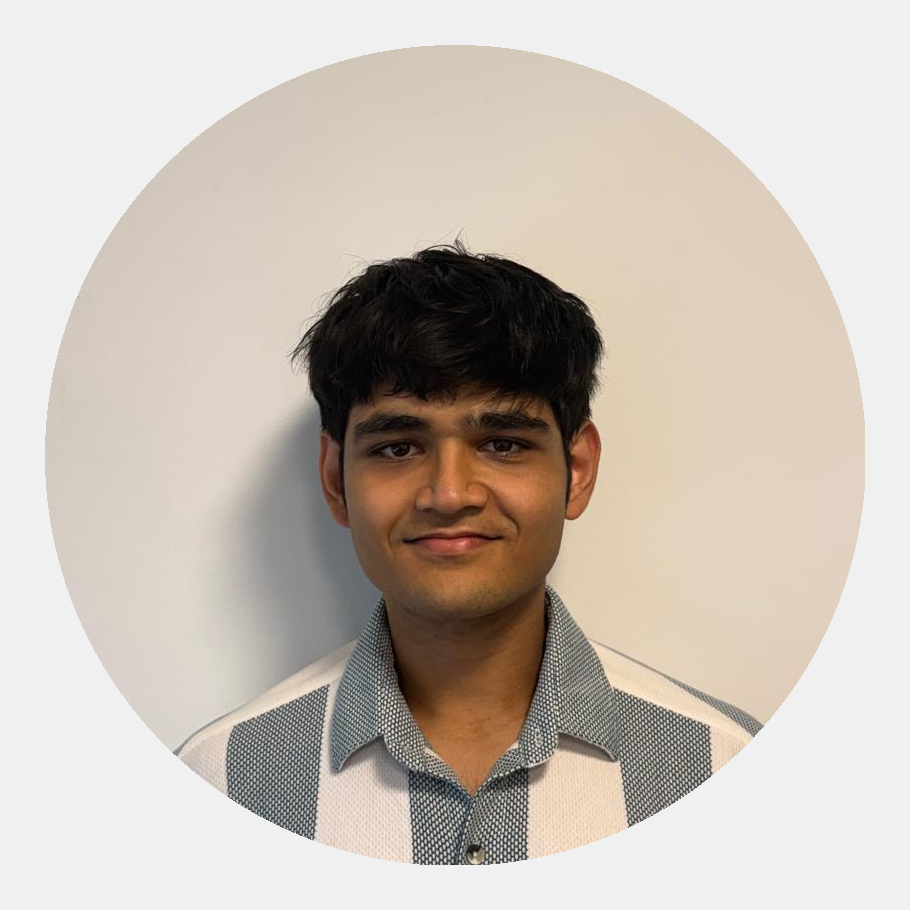
\includegraphics[width=2.92cm]{profile.png}};
    \draw[ringcol,line width=1.4pt] (0,0) circle (1.26cm);
  \end{tikzpicture}
\end{minipage}

\vspace{4pt}
\noindent\textcolor{rulecol}{\rule{\bodyw}{0.5pt}}
\par\vspace{4pt}
\noindent{\fontsize{8.4}{10.5}\selectfont
\contactitem{\faPhone*}{+91 93216 69960}\hfill
\contactitem{\faEnvelope}{\href{mailto:kamdardhruv8@gmail.com}{kamdardhruv8@gmail.com}}\hfill
\contactitem{\faMapMarker*}{Mumbai, India}\hfill
\contactitem{\faLinkedin}{\href{https://www.linkedin.com/in/dhruv-kamdar-254472363/}{linkedin.com/in/dhruv-kamdar}}\hfill
\contactitem{\faGlobe}{\href{https://kamdardhruv8-droid.github.io/}{kamdardhruv8-droid.github.io}}}
\par\vspace{1pt}
\noindent\textcolor{rulecol}{\rule{\bodyw}{0.5pt}}

% ============================== PROFILE ======================================
\mnhead{Professional Profile}
{\fontsize{8.75}{10.8}\selectfont
MSc Finance Analytics graduate combining financial domain knowledge with hands-on analytics
and applied AI. Strong across the analytics cycle --- cleaning, validation, exploratory
analysis, statistical modelling and dashboard reporting in Python, SQL, R and Excel --- and in
automating research and reporting workflows with agentic AI tooling. Comfortable presenting
technical findings to senior, non-technical stakeholders. Seeking data analyst, AI and
financial analytics roles in India.\par}

% ============================== EXPERIENCE ===================================
\mnhead{Experience}

\job{Student Consultant --- Research Lead}{Practera Finance Micro Internship, London, UK}{Jun 2026 -- Jul 2026}
\begin{cvbullets}
\item Analysed \$77B+ of financial data from multiple sources to identify investment trends,
      uncovering an insight that redirected the team's entire recommendation approach.
\item Validated and reconciled data with an 8-person cross-functional team, ensuring quality
      and consistency across all deliverables.
\item Presented recommendations directly to the client's Managing Director, translating
      complex analysis into clear, actionable insight.
\item Managed four concurrent workstreams to deadline, adapting the approach when initial
      assumptions proved flawed.
\end{cvbullets}

\vspace{1pt}
\job{Intern --- Data \& Systems}{DG Software, Mumbai, India}{Mar 2025 -- Aug 2025}
\begin{cvbullets}
\item Improved data integrity by 30\% across 12 database tables by redesigning the data
      architecture and automating validation.
\item Wrote SQL to query, extract, validate and reconcile datasets of 10,000+ records,
      improving retrieval efficiency by 25\%.
\item Built reporting dashboards used by senior management for operational decisions,
      eliminating 8+ hours of weekly manual processing.
\end{cvbullets}

% ============================== PROJECTS =====================================
\mnhead{Analytics, AI \& Finance Projects}

\job{Systematic Trading Strategy --- MSc Dissertation}{King's College London}{2026}
\begin{cvbullets}
\item Built and backtested a systematic trading strategy in Python on large historical market data, evaluating signal quality and risk-adjusted returns.
\end{cvbullets}

\vspace{1pt}
\job{Agentic AI Workflow Automation}{Personal project}{Jun 2026 -- Present}
\begin{cvbullets}
\item Built automated pipelines in Python, n8n and LangGraph for retrieval, validation and report generation, cutting research from hours to minutes.
\end{cvbullets}

\vspace{1pt}
\job{Team Leader --- King's Investment Fund}{Equity portfolio, UK \& European markets}{Mar 2026 -- Jun 2026}
\begin{cvbullets}
\item Led an 8-member team; delivered +300 to +500 bps outperformance versus the FTSE 100
      by applying CAPM and factor analysis to evaluate risk-adjusted returns.
\item Built performance dashboards in Python and Excel; presented strategy
      recommendations to faculty advisors.
\end{cvbullets}

\vspace{1pt}
\job{Forage Virtual Experience Programmes}{Quantium --- retail analytics \ \textbar\ \ Goldman Sachs --- investment banking operations}{Aug 2026}
\begin{cvbullets}
\item \textbf{Quantium:} cleaned and analysed 264,000+ retail transaction records in R and
      Python --- customer segmentation, brand affinity and experiment design, delivered as a
      client-ready report.
\item \textbf{Goldman Sachs:} analysed trade settlement data across Trading, Compliance and Technology teams, documenting process controls.
\end{cvbullets}

% ============================== EDUCATION ====================================
\mnhead{Education}

\job{MSc Finance Analytics}{King's College London, United Kingdom}{Sep 2025 -- Sep 2026}
{\fontsize{8.5}{10.2}\selectfont
\textbf{Modules:} Econometrics, Statistical Modelling, Data Analytics, Big Data \& Text
Analytics, Financial Reporting\par}

\vspace{4pt}
\job{Bachelor of Commerce (B.Com.) --- GPA 8.7/10}{Jai Hind College, University of Mumbai, India}{Mar 2022 -- Mar 2025}

% ============================== SKILLS =======================================
\mnhead{Technical Skills \& Certifications}
\skillrow{Programming \& Data}{Python (Pandas, NumPy, Matplotlib), SQL (querying, joins, validation), R, Advanced Excel (PivotTables, VLOOKUP)}
\skillrow{AI \& Automation}{Agentic AI workflows, LangGraph, n8n, LLM-assisted research automation, Git}
\skillrow{Analytics \& BI}{Data cleaning \& validation, exploratory analysis, statistical modelling \& inference, A/B testing, customer segmentation, dashboard design \& data visualisation, process automation}
\skillrow{Finance}{Bloomberg Terminal, portfolio \& risk analysis (CAPM, factor models), equity research, financial reporting}
\skillrow{Certifications}{DeepLearning.AI --- Agentic AI Certificate; Forage --- Goldman Sachs Operations, Quantium Data Analytics}

\end{document}
